\documentclass[aspectratio=169,12pt,t]{beamer}

% --- Theme: Metropolis (modern, clean) ---
\usetheme[progressbar=frametitle,numbering=fraction,block=fill]{metropolis}

% --- Fira Sans font (install texlive-fonts-extra if missing) ---
\IfFileExists{FiraSans.sty}{\usepackage[sfdefault]{FiraSans}}{}

% --- Light background with warm accent ---
\definecolor{mDarkTeal}{RGB}{35,55,59}
\definecolor{mLightBrown}{RGB}{235,228,216}
\definecolor{mAccent}{RGB}{140,70,20}

\setbeamercolor{normal text}{fg=mDarkTeal,bg=white}
\setbeamercolor{alerted text}{fg=mAccent}
\setbeamercolor{frametitle}{bg=mDarkTeal,fg=white}
\setbeamercolor{progress bar}{fg=mAccent,bg=mLightBrown}
\setbeamercolor{title separator}{fg=mAccent}
\setbeamercolor{progress bar in head/foot}{fg=mAccent,bg=mLightBrown}
\setbeamercolor{progress bar in section page}{fg=mAccent,bg=mLightBrown}

% --- Packages ---
\usepackage[utf8]{inputenc}
\usepackage{amsmath,amssymb,amsthm}
\usepackage{mathrsfs}
\usepackage{tikz}
\usetikzlibrary{arrows.meta,positioning,calc,decorations.pathreplacing,shapes,patterns}
\usepackage{pgfplots}
\pgfplotsset{compat=1.18}

% --- Semi-transparent white highlight for text on top of background images ---
\usepackage[most]{tcolorbox}

% Inline highlight: \hl{short text}
\newtcbox{\hl}{%
  nobeforeafter, tcbox raise base,
  colback=white, opacityback=0.6,
  colframe=white, opacityframe=0,
  sharp corners, boxsep=2pt, left=3pt, right=3pt, top=2pt, bottom=2pt%
}

% Block highlight: \begin{hlbox} ... \end{hlbox}  (multi-line, paragraphs, itemize)
% Optional argument accepts any tcolorbox key, e.g. [width=0.6\linewidth]
\newtcolorbox{hlbox}[1][]{%
  enhanced, breakable,
  colback=white, opacityback=0.6,
  colframe=white, opacityframe=0,
  boxsep=3pt, left=6pt, right=6pt, top=4pt, bottom=4pt,
  sharp corners,
  {#1}%
}

% --- Custom colors for content types ---
\definecolor{defcolor}{RGB}{25,85,120}
\definecolor{thmcolor}{RGB}{140,35,35}
\definecolor{proofcolor}{RGB}{35,100,50}
\definecolor{excolor}{RGB}{140,75,10}
\definecolor{remcolor}{RGB}{90,90,90}

% --- Beamer blocks for mathematical content types (semi-transparent) ---
% Native Beamer blocks cannot carry an alpha channel, so we render the blocks
% with tcolorbox instead. Title and body are both at 50% opacity; body tint
% bumped from !5 to !15 to stay visible after the alpha is applied.
\tcbset{hlblockbase/.style={
  enhanced, breakable,
  coltitle=white, fonttitle=\bfseries,
  opacitybacktitle=0.8, opacityback=0.6,
  opacityframe=0,
  sharp corners,
  boxsep=1pt, left=5pt, right=5pt, top=2pt, bottom=2pt,
  toptitle=1pt, bottomtitle=1pt
}}

\newtcolorbox{defblock}[1]{hlblockbase, title={#1},
  colbacktitle=defcolor, colback=defcolor!15, colframe=defcolor}
\newtcolorbox{thmblock}[1]{hlblockbase, title={#1},
  colbacktitle=thmcolor, colback=thmcolor!15, colframe=thmcolor}
\newtcolorbox{proofblock}[1]{hlblockbase, title={#1},
  colbacktitle=proofcolor, colback=proofcolor!15, colframe=proofcolor}
\newtcolorbox{exblock}[1]{hlblockbase, title={#1},
  colbacktitle=excolor, colback=excolor!15, colframe=excolor}
\newtcolorbox{remblock}[1]{hlblockbase, title={#1},
  colbacktitle=remcolor, colback=remcolor!15, colframe=remcolor}

% --- Metadata ---
\title{Chapter 1: The Real and Complex Number Systems}
\subtitle{Section: Introduction}
\author{Based on Walter Rudin's \emph{Principles of Mathematical Analysis}}
\date{}

\begin{document}

{
\usebackgroundtemplate{%
  
\includegraphics[width=\paperwidth,height=\paperheight,keepaspectratio=false]{chapter_01_bg_00.png}%
}
% ============================================================
% TITLE AND OUTLINE
% ============================================================
\begin{frame}
  \titlepage

  \note{
    Welcome to the Principles of Mathematical Analysis video series. This is Chapter 1: The Real and Complex Number Systems. In this first section, called Introduction, we will explore why the rational numbers are not sufficient for doing analysis, and why we need to construct the real number system. Let's get started.
  }
\end{frame}
}

{
\usebackgroundtemplate{%
  
\includegraphics[width=\paperwidth,height=\paperheight,keepaspectratio=false]{chapter_01_bg_01.png}%
}
% ============================================================
\begin{frame}[c]{Outline}
  \begin{center}
    \tableofcontents
  \end{center}

  \note{
    Here is an outline of what we will cover. We start with the motivation for why the rationals are inadequate. Then we work through Example 1.1, which proves that the square root of 2 is irrational and reveals a gap in the rational numbers. Next, Remark 1.2 explains the significance of these gaps. Finally, we introduce the basic set-theoretic definitions that will be used throughout the book. Let's begin with the motivation.
  }
\end{frame}

% ============================================================
% MOTIVATION (progressive build)
% ============================================================
\section{Motivation}

% --- Build 1/3: Analysis needs precise numbers ---
\begin{frame}{Why This Section Matters}
  \begin{hlbox}
    \begin{itemize}
      \item Analysis requires a \alert{precisely defined} number concept
    \end{itemize}
  \end{hlbox}

  \note{
    We begin with a fundamental observation. A satisfactory discussion of the main concepts of analysis, things like convergence, continuity, differentiation, and integration, must be based on an accurately defined number concept. We cannot just rely on intuition about numbers; we need a rigorous foundation.
  }
\end{frame}

% --- Build 2/3: Q is not enough ---
\begin{frame}{Why This Section Matters}
  \begin{hlbox}
    \begin{itemize}
      \item Analysis requires a \alert{precisely defined} number concept
      \item The rational numbers $\mathbb{Q}$ are \emph{not enough}
    \end{itemize}
  \end{hlbox}

  \note{
    The rational numbers, fractions of the form "m" over "n", might seem like a natural candidate for this foundation. But it turns out that the rational number system is inadequate for many purposes, both as an algebraic structure and as an ordered set. There are fundamental gaps in the rationals that prevent us from doing analysis properly. Let's see the most striking example of this.
  }
\end{frame}

% --- Build 3/3: Goal and preview ---
\begin{frame}{Why This Section Matters}
  \begin{hlbox}
    \begin{itemize}
      \item Analysis requires a \alert{precisely defined} number concept
      \item The rational numbers $\mathbb{Q}$ are \emph{not enough}
      \item Goal: understand the \alert{gaps} in $\mathbb{Q}$ that force us to build $\mathbb{R}$
    \end{itemize}

    \vspace{1em}
    \textbf{Main ideas in this section:}
    \begin{itemize}
      \item $\sqrt{2}$ is irrational (Example 1.1)
      \item The rationals have gaps that the reals fill (Remark 1.2)
      \item Basic set-theoretic language (Definitions 1.3--1.4)
    \end{itemize}
  \end{hlbox}

  \note{
    Our goal in this section is to understand exactly what these gaps are and why they force us to construct the real number system. We will do this through three main ideas: first, we will prove that the square root of 2 is irrational in Example 1.1; second, Remark 1.2 will explain why this means the rationals have gaps that the reals fill; and third, we will introduce the basic set-theoretic language in Definitions 1.3 and 1.4 that the rest of the book depends on.
  }
\end{frame}

% ============================================================
% THE PROBLEM WITH RATIONALS (progressive build)
% ============================================================

% --- Build 1/3: Starting point ---
\begin{frame}{The Problem with Rationals}
  \begin{hlbox}
    We assume familiarity with $\mathbb{Q} = \{m/n : m, n \in \mathbb{Z},\; n \neq 0\}$.

    \vspace{1em}
    $\mathbb{Q}$ is inadequate as both a \alert{field} and an \alert{ordered set}.
  \end{hlbox}

  \note{
    Rudin opens the book by stating that we will not go all the way back to the axioms for the integers. We take the rational numbers as given. The rationals are the numbers of the form "m" over "n", where "m" and "n" are integers and "n" is not zero. Now, the rational number system turns out to be inadequate in two senses: as a field, meaning the algebraic structure for doing arithmetic, and as an ordered set, meaning the structure for comparing numbers. These terms will be defined precisely in later sections.
  }
\end{frame}

% --- Build 2/3: Key example ---
\begin{frame}{The Problem with Rationals}
  \begin{hlbox}
    We assume familiarity with $\mathbb{Q} = \{m/n : m, n \in \mathbb{Z},\; n \neq 0\}$.

    \vspace{1em}
    $\mathbb{Q}$ is inadequate as both a \alert{field} and an \alert{ordered set}.

    \vspace{1em}
    \textbf{Key example:} There is no $p \in \mathbb{Q}$ with $p^2 = 2$.

    \vspace{0.5em}
    The sequence $1,\; 1.4,\; 1.41,\; 1.414,\; 1.4142,\; \dots$ ``tends to $\sqrt{2}$''
  \end{hlbox}

  \note{
    The striking illustration of this inadequacy is that there is no rational number whose square equals 2. We can write down better and better decimal approximations: 1, 1.4, 1.41, 1.414, 1.4142, and so on. This sequence seems to tend toward the square root of 2. But this raises a deep question.
  }
\end{frame}

% --- Build 3/3: The fundamental question ---
\begin{frame}{The Problem with Rationals}
  \begin{hlbox}
    We assume familiarity with $\mathbb{Q} = \{m/n : m, n \in \mathbb{Z},\; n \neq 0\}$.

    \vspace{1em}
    $\mathbb{Q}$ is inadequate as both a \alert{field} and an \alert{ordered set}.

    \vspace{1em}
    \textbf{Key example:} There is no $p \in \mathbb{Q}$ with $p^2 = 2$.

    \vspace{0.5em}
    The sequence $1,\; 1.4,\; 1.41,\; 1.414,\; 1.4142,\; \dots$ ``tends to $\sqrt{2}$''
  \end{hlbox}

  \vspace{0.5em}
  \begin{center}
    \hl{\alert{But what \emph{is} $\sqrt{2}$ if we only have $\mathbb{Q}$?}}
  \end{center}

  \note{
    But if we have not yet defined the real numbers, then what exactly is this sequence tending to? The square root of 2 is not a rational number, so it does not exist in our number system. This question can only be answered once we construct the real number system. Let's first prove rigorously that the square root of 2 is indeed irrational.
  }
\end{frame}
}

{
\usebackgroundtemplate{%
  
\includegraphics[width=\paperwidth,height=\paperheight,keepaspectratio=false]{chapter_01_bg_02.png}%
}
% ============================================================
% EXAMPLE 1.1 (progressive build)
% ============================================================
\section{Example 1.1: Irrationality of $\sqrt{2}$}

% --- Setup Build 1/2: Statement ---
\begin{frame}{Example 1.1: $\sqrt{2}$ Is Irrational --- Setup}
  \begin{exblock}{Example 1.1}
    The equation
    \begin{equation}
      p^2 = 2 \tag{1}
    \end{equation}
    is not satisfied by any rational $p$.
  \end{exblock}

  \vspace{0.5em}
  \hl{\textbf{Technique:} Proof by contradiction}

  \note{
    Here is the precise statement of Example 1.1: the equation "p" squared equals 2 is not satisfied by any rational number "p". In other words, the square root of 2 is irrational. This is a classic result, and we will prove it using the technique of proof by contradiction. We assume that such a rational "p" exists, and then show that this leads to an impossible conclusion.
  }
\end{frame}

% --- Setup Build 2/2: Assumption and consequence ---
\begin{frame}{Example 1.1: $\sqrt{2}$ Is Irrational --- Setup}
  \begin{exblock}{Example 1.1}
    The equation
    \begin{equation}
      p^2 = 2 \tag{1}
    \end{equation}
    is not satisfied by any rational $p$.
  \end{exblock}

  \vspace{0.5em}
  \begin{hlbox}
    \textbf{Technique:} Proof by contradiction

    \vspace{0.5em}
    \textbf{Assume} $p = m/n$ with $m, n \in \mathbb{Z}$, not both even.

    Then (1) gives:
    \begin{equation}
      m^2 = 2n^2 \tag{2}
    \end{equation}
  \end{hlbox}

  \note{
    Suppose for contradiction there were such a rational "p". Then we could write "p" as "m" over "n", where "m" and "n" are integers. Moreover, we can assume that "m" and "n" are not both even, because if they were, we could cancel common factors of 2 until at least one of them is odd. Now, if "p" squared equals 2, and "p" equals "m" over "n", then squaring both sides gives "m" squared over "n" squared equals 2, which means "m" squared equals 2 "n" squared. This is equation 2 on the slide.
  }
\end{frame}

% --- Contradiction Build 1/3: m is even ---
\begin{frame}{Example 1.1: $\sqrt{2}$ Is Irrational --- The Contradiction}
  \begin{hlbox}
    From $m^2 = 2n^2$:

    \vspace{0.5em}
    \begin{enumerate}
      \item $m^2$ is even $\;\Longrightarrow\;$ $m$ is even
    \end{enumerate}
  \end{hlbox}

  \note{
    Now we chase the consequences of equation 2. Since "m" squared equals 2 "n" squared, we see that "m" squared is even. But if "m" were odd, then "m" squared would also be odd. So "m" must be even. Let's see what this tells us about "m" squared.
  }
\end{frame}

% --- Contradiction Build 2/3: 4 divides m² ---
\begin{frame}{Example 1.1: $\sqrt{2}$ Is Irrational --- The Contradiction}
  \begin{hlbox}
    From $m^2 = 2n^2$:

    \vspace{0.5em}
    \begin{enumerate}
      \item $m^2$ is even $\;\Longrightarrow\;$ $m$ is even
      \item $m$ even $\;\Longrightarrow\;$ $m^2$ divisible by $4$
    \end{enumerate}
  \end{hlbox}

  \note{
    Since "m" is even, we can write "m" as 2 "k" for some integer "k". Then "m" squared equals 4 "k" squared, which means "m" squared is divisible by 4, not just by 2. This extra factor of 2 is what we will exploit in the next step to show that "n" must also be even.
  }
\end{frame}

% --- Contradiction Build 3/3: n is even ---
\begin{frame}{Example 1.1: $\sqrt{2}$ Is Irrational --- The Contradiction}
  \begin{hlbox}
    From $m^2 = 2n^2$:

    \vspace{0.5em}
    \begin{enumerate}
      \item $m^2$ is even $\;\Longrightarrow\;$ $m$ is even
      \item $m$ even $\;\Longrightarrow\;$ $m^2$ divisible by $4$
      \item $m^2 = 2n^2$ and $4 \mid m^2$ $\;\Longrightarrow\;$ $2 \mid n^2$ $\;\Longrightarrow\;$ $n$ is even
    \end{enumerate}
  \end{hlbox}

  \note{
    Looking back at equation 2, we have "m" squared equals 2 "n" squared, and since 4 divides "m" squared, it follows that 2 divides "n" squared. But then "n" squared is even, which forces "n" to be even as well.
  }
\end{frame}

% --- Contradiction Build 4/4: Conclusion ---
\begin{frame}{Example 1.1: $\sqrt{2}$ Is Irrational --- The Contradiction}
  \begin{hlbox}
    From $m^2 = 2n^2$:

    \vspace{0.5em}
    \begin{enumerate}
      \item $m^2$ is even $\;\Longrightarrow\;$ $m$ is even
      \item $m$ even $\;\Longrightarrow\;$ $m^2$ divisible by $4$
      \item $m^2 = 2n^2$ and $4 \mid m^2$ $\;\Longrightarrow\;$ $2 \mid n^2$ $\;\Longrightarrow\;$ $n$ is even
    \end{enumerate}

    \vspace{1em}
    \begin{center}
      Both $m$ and $n$ are even --- \alert{contradicts} our assumption!
    \end{center}

    \vspace{0.5em}
    $\boxed{\text{No rational } p \text{ satisfies } p^2 = 2.}$
  \end{hlbox}

  \note{
    So both "m" and "n" are even. But we specifically chose "m" and "n" so that they are not both even! This is a contradiction. Therefore, our assumption was wrong, and no rational "p" can satisfy "p" squared equals 2. The square root of 2 is irrational. Now let us examine this situation more closely.
  }
\end{frame}

% ============================================================
% SETS A AND B (progressive build)
% ============================================================

% --- Build 1/3: Define A and B ---
\begin{frame}{Example 1.1: The Sets $A$ and $B$}
  \begin{hlbox}
    Define two subsets of positive rationals:
    \[
      A = \{p \in \mathbb{Q}^{+} : p^2 < 2\}, \qquad B = \{p \in \mathbb{Q}^{+} : p^2 > 2\}
    \]
  \end{hlbox}

  \note{
    Now Rudin examines the situation more closely. He defines two sets of positive rationals. The set "A" consists of all positive rationals "p" whose square is less than 2, and the set "B" consists of all positive rationals "p" whose square is greater than 2. These sets partition the positive rationals into two groups: those to the left of the square root of 2, and those to the right.
  }
\end{frame}

% --- Build 2/3: Diagram ---
\begin{frame}{Example 1.1: The Sets $A$ and $B$}
  \begin{hlbox}
    Define two subsets of positive rationals:
    \[
      A = \{p \in \mathbb{Q}^{+} : p^2 < 2\}, \qquad B = \{p \in \mathbb{Q}^{+} : p^2 > 2\}
    \]
  \end{hlbox}

  \vspace{0.5em}
  \begin{center}
  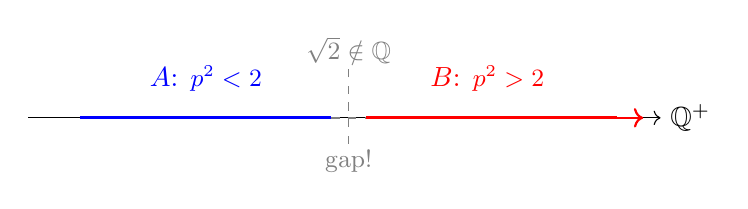
\begin{tikzpicture}[scale=1.1]
    \draw[->] (-0.3,0) -- (7,0) node[right]{$\mathbb{Q}^{+}$};
    \draw[very thick, blue] (0.3,0) -- (3.2,0);
    \node[blue, above=6pt] at (1.75,0) {$A$: \small $p^2 < 2$};
    \draw[very thick, red] (3.6,0) -- (6.5,0);
    \draw[red, ->, thick] (6.5,0) -- (6.8,0);
    \node[red, above=6pt] at (5.0,0) {$B$: \small $p^2 > 2$};
    \draw[thick, dashed, gray] (3.2,0) -- (3.6,0);
    \node[gray, below=8pt] at (3.4,0) {\small gap!};
    \draw[gray, dashed] (3.4,-0.3) -- (3.4,0.6);
    \node[gray, above=16pt] at (3.4,0) {\small $\sqrt{2} \notin \mathbb{Q}$};
  \end{tikzpicture}
  \end{center}

  \note{
    As you can see on the diagram, "A" lies to the left and "B" lies to the right on the number line, with a gap in between where the square root of 2 should be. But since the square root of 2 is not rational, it does not belong to either set. There is a genuine hole between "A" and "B".
  }
\end{frame}

% --- Build 3/3: The claim ---
\begin{frame}{Example 1.1: The Sets $A$ and $B$}
  \begin{hlbox}
    Define two subsets of positive rationals:
    \[
      A = \{p \in \mathbb{Q}^{+} : p^2 < 2\}, \qquad B = \{p \in \mathbb{Q}^{+} : p^2 > 2\}
    \]
  \end{hlbox}

  \vspace{0.5em}
  \begin{center}
  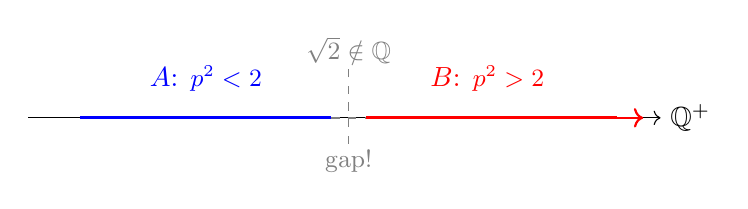
\begin{tikzpicture}[scale=1.1]
    \draw[->] (-0.3,0) -- (7,0) node[right]{$\mathbb{Q}^{+}$};
    \draw[very thick, blue] (0.3,0) -- (3.2,0);
    \node[blue, above=6pt] at (1.75,0) {$A$: \small $p^2 < 2$};
    \draw[very thick, red] (3.6,0) -- (6.5,0);
    \draw[red, ->, thick] (6.5,0) -- (6.8,0);
    \node[red, above=6pt] at (5.0,0) {$B$: \small $p^2 > 2$};
    \draw[thick, dashed, gray] (3.2,0) -- (3.6,0);
    \node[gray, below=8pt] at (3.4,0) {\small gap!};
    \draw[gray, dashed] (3.4,-0.3) -- (3.4,0.6);
    \node[gray, above=16pt] at (3.4,0) {\small $\sqrt{2} \notin \mathbb{Q}$};
  \end{tikzpicture}
  \end{center}

  \vspace{0.3em}
  \begin{hlbox}
    \alert{Claim:} $A$ has no largest element, and $B$ has no smallest element.
  \end{hlbox}

  \note{
    The crucial claim is that "A" has no largest element and "B" has no smallest element. This means there is no rational number sitting right at the boundary of this gap. No matter how close you get to the square root of 2 from either side, you can always get closer while staying within the rationals. The gap is real and cannot be plugged using rationals alone. Let's see how Rudin proves this claim.
  }
\end{frame}

% ============================================================
% KEY CONSTRUCTION (progressive build)
% ============================================================

% --- Build 1/2: Define q ---
\begin{frame}{Example 1.1: The Key Construction}
  \begin{hlbox}
    For each rational $p > 0$, define:
    \begin{equation}
      q = p - \frac{p^2 - 2}{p + 2} = \frac{2p + 2}{p + 2} \tag{3}
    \end{equation}
  \end{hlbox}

  \note{
    To prove the claim, Rudin introduces a clever construction. Given any positive rational "p", he defines a new rational "q" by the formula: "q" equals "p" minus the quantity "p" squared minus 2, divided by "p" plus 2. This simplifies to 2 "p" plus 2, all divided by "p" plus 2. The idea is that "q" is a rational number that is closer to the square root of 2 than "p" is, while remaining on the same side of the square root of 2 as "p". Let's see why this works.
  }
\end{frame}

% --- Build 2/2: Key identity ---
\begin{frame}{Example 1.1: The Key Construction}
  \begin{hlbox}
    For each rational $p > 0$, define:
    \begin{equation}
      q = p - \frac{p^2 - 2}{p + 2} = \frac{2p + 2}{p + 2} \tag{3}
    \end{equation}

    Then:
    \begin{equation}
      q^2 - 2 = \frac{2(p^2 - 2)}{(p+2)^2} \tag{4}
    \end{equation}

    \vspace{0.5em}
    \textbf{Key observation:} $q^2 - 2$ has the \alert{same sign} as $p^2 - 2$.
  \end{hlbox}

  \note{
    The crucial algebraic identity, equation 4, shows that "q" squared minus 2 equals 2 times "p" squared minus 2, divided by "p" plus 2 squared. Since "p" plus 2 squared is always positive, this tells us that "q" squared minus 2 has the same sign as "p" squared minus 2. This is the engine that drives the whole argument. If "p" is in "A", then "q" will also be in "A". If "p" is in "B", then "q" will also be in "B".
  }
\end{frame}

% ============================================================
% COMPLETING THE ARGUMENT (progressive build)
% ============================================================

% --- Build 1/3: Case 1 ---
\begin{frame}{Example 1.1: Completing the Argument}
  \begin{hlbox}
    \textbf{Case 1:} $p \in A$ (so $p^2 < 2$, i.e., $p^2 - 2 < 0$)
    \begin{itemize}
      \item From (3): $q > p$ \quad {\small (subtracting a negative number)}
      \item From (4): $q^2 - 2 < 0$, so $q^2 < 2$
      \item Thus $q \in A$ and $q > p$ \quad $\Longrightarrow$ \quad \alert{$p$ is not the largest in $A$}
    \end{itemize}
  \end{hlbox}

  \note{
    Let's apply the construction. First, suppose "p" is in "A", meaning "p" squared is less than 2. Then "p" squared minus 2 is negative. Looking at equation 3, we are subtracting a negative number from "p", so "q" is greater than "p". And from equation 4, "q" squared minus 2 is also negative, meaning "q" squared is less than 2, so "q" is also in "A". We have found a rational in "A" that is strictly larger than "p", so "p" cannot be the largest element of "A".
  }
\end{frame}

% --- Build 2/3: Case 2 ---
\begin{frame}{Example 1.1: Completing the Argument}
  \begin{hlbox}
    \textbf{Case 1:} $p \in A$ (so $p^2 < 2$, i.e., $p^2 - 2 < 0$)
    \begin{itemize}
      \item From (3): $q > p$ \quad {\small (subtracting a negative number)}
      \item From (4): $q^2 - 2 < 0$, so $q^2 < 2$
      \item Thus $q \in A$ and $q > p$ \quad $\Longrightarrow$ \quad \alert{$p$ is not the largest in $A$}
    \end{itemize}

    \vspace{0.5em}
    \textbf{Case 2:} $p \in B$ (so $p^2 > 2$, i.e., $p^2 - 2 > 0$)
    \begin{itemize}
      \item From (3): $0 < q < p$ \quad {\small (subtracting a positive number)}
      \item From (4): $q^2 - 2 > 0$, so $q^2 > 2$
      \item Thus $q \in B$ and $q < p$ \quad $\Longrightarrow$ \quad \alert{$p$ is not the smallest in $B$}
    \end{itemize}
  \end{hlbox}

  \note{
    Now suppose "p" is in "B", meaning "p" squared is greater than 2. Then "p" squared minus 2 is positive. From equation 3, "q" is less than "p" but still positive. From equation 4, "q" squared minus 2 is positive, so "q" is in "B". We have found a rational in "B" strictly smaller than "p", so "p" is not the smallest element of "B". Now let's put these two cases together.
  }
\end{frame}

% --- Build 3/3: Conclusion ---
\begin{frame}{Example 1.1: Completing the Argument}
  \begin{hlbox}
    \textbf{Case 1:} $p \in A$  (so $p^2 < 2$, i.e., $p^2 - 2 < 0$)
    \begin{itemize}
      \item From (3): $q > p$ \quad {\small (subtracting a negative number)}
      \item From (4): $q^2 - 2 < 0$, so $q^2 < 2$
      \item Thus $q \in A$ and $q > p$ \quad $\Longrightarrow$ \quad \alert{$p$ is not the largest in $A$}
    \end{itemize}

    \vspace{0.5em}
    \textbf{Case 2:} $p \in B$ (so $p^2 > 2$, i.e., $p^2 - 2 > 0$)
    \begin{itemize}
      \item From (3): $0 < q < p$ \quad {\small (subtracting a positive number)}
      \item From (4): $q^2 - 2 > 0$, so $q^2 > 2$
      \item Thus $q \in B$ and $q < p$ \quad $\Longrightarrow$ \quad \alert{$p$ is not the smallest in $B$}
    \end{itemize}

    \vspace{0.5em}
    $\boxed{A \text{ has no largest element, } B \text{ has no smallest element.}}$
  \end{hlbox}

  \note{
    Since "p" was arbitrary in each case, "A" has no maximum and "B" has no minimum. This is the gap in the rationals. There is no rational number at the boundary between "A" and "B". The square root of 2 should be there, but it simply does not exist in the rational number system.
  }
\end{frame}
}

{
\usebackgroundtemplate{%
  
\includegraphics[width=\paperwidth,height=\paperheight,keepaspectratio=false]{chapter_01_bg_03.png}%
}
% ============================================================
% REMARK 1.2 (progressive build)
% ============================================================
\section{Remark 1.2: Gaps in the Rationals}

% --- Build 1/2: Density ---
\begin{frame}{Remark 1.2: Gaps in $\mathbb{Q}$}
  \begin{remblock}{Remark 1.2}
    The rational number system has \alert{gaps}, despite the fact that between any two rationals there is another:
    \[
      r < s \;\Longrightarrow\; r < \frac{r+s}{2} < s
    \]
  \end{remblock}

  \note{
    Remark 1.2 captures the philosophical lesson of Example 1.1. The rationals are dense: between any two rationals "r" and "s", the average "r" plus "s" over 2 is another rational strictly between them. So in some sense, the rationals are spread everywhere on the number line. Yet they still have gaps. The set "A" has no maximum, the set "B" has no minimum, and there is nothing in the rationals sitting between them.
  }
\end{frame}

% --- Build 2/2: R fills the gaps ---
\begin{frame}{Remark 1.2: Gaps in $\mathbb{Q}$}
  \begin{remblock}{Remark 1.2}
    The rational number system has \alert{gaps}, despite the fact that between any two rationals there is another:
    \[
      r < s \;\Longrightarrow\; r < \frac{r+s}{2} < s
    \]
  \end{remblock}

  \vspace{1em}
  \begin{hlbox}
    The \alert{real number system} fills these gaps --- the principal reason $\mathbb{R}$ is fundamental to analysis.
  \end{hlbox}

  \note{
    The real number system is specifically designed to fill these gaps. This gap-filling property, which we will later call the least upper bound property, is the principal reason that the reals are the right setting for analysis. To precisely describe the structure of the reals, we first need to discuss the general concepts of ordered sets and fields, which is what the rest of Chapter 1 will do. But before we move on to those topics, let us set up some basic set-theoretic notation that will be used throughout the entire book.
  }
\end{frame}
}

{
\usebackgroundtemplate{%
  
\includegraphics[width=\paperwidth,height=\paperheight,keepaspectratio=false]{chapter_01_bg_04.png}%
}
% ============================================================
% DEFINITIONS 1.3--1.4 (progressive build)
% ============================================================
\section{Definitions 1.3--1.4: Set-Theoretic Terminology}

% --- Build 1/4: Membership ---
\begin{frame}{Definition 1.3: Basic Set Notation}
  \begin{defblock}{Definition 1.3: Set Membership}
    \begin{itemize}
      \item $x \in A$: \quad $x$ is a \emph{member} (element) of $A$
      \item $x \notin A$: \quad $x$ is not a member of $A$
    \end{itemize}
  \end{defblock}

  \note{
    Now Rudin introduces the standard set-theoretic terminology that will be used throughout the book. If "A" is any set, whose elements may be numbers or any other objects, we write "x" belongs to "A" to indicate that "x" is a member, or element, of "A". If "x" is not a member of "A", we write "x" does not belong to "A".
  }
\end{frame}

% --- Build 2/4: Empty set ---
\begin{frame}{Definition 1.3: Basic Set Notation}
  \begin{defblock}{Definition 1.3: Set Membership and the Empty Set}
    \begin{itemize}
      \item $x \in A$: \quad $x$ is a \emph{member} (element) of $A$
      \item $x \notin A$: \quad $x$ is not a member of $A$
      \item The set with no elements is the \alert{empty set}, denoted $\emptyset$
      \item A set with at least one element is called \alert{nonempty}
    \end{itemize}
  \end{defblock}

  \note{
    The set which contains no element will be called the empty set, denoted by the symbol that looks like a zero with a slash through it. If a set has at least one element, it is called nonempty. The empty set is a perfectly valid set in mathematics; it just happens to have nothing in it. It may seem like a trivial concept, but the empty set plays an important role in many definitions and arguments throughout analysis. Next, we define the notion of a subset.
  }
\end{frame}

% --- Build 3/4: Subsets ---
\begin{frame}{Definition 1.3: Basic Set Notation}
  \begin{defblock}{Definition 1.3: Set Membership and the Empty Set}
    \begin{itemize}
      \item $x \in A$: \quad $x$ is a \emph{member} (element) of $A$
      \item $x \notin A$: \quad $x$ is not a member of $A$
      \item The set with no elements is the \alert{empty set}, denoted $\emptyset$
      \item A set with at least one element is called \alert{nonempty}
    \end{itemize}
  \end{defblock}

  \vspace{0.5em}
  \begin{defblock}{Definition 1.3 (cont.): Subsets}
    \begin{itemize}
      \item $A \subset B$: \quad every element of $A$ is an element of $B$ \\ {\small ($A$ is a \emph{subset} of $B$)}
      \item If also $\exists\, b \in B$ with $b \notin A$: \quad $A$ is a \alert{proper subset} of $B$
      \item $A \subset A$ for every set $A$
    \end{itemize}
  \end{defblock}

  \note{
    Next, if "A" and "B" are sets, and if every element of "A" is an element of "B", we say that "A" is a subset of "B", and write "A" subset "B". If in addition there is an element of "B" which is not in "A", then "A" is said to be a proper subset of "B". Note that "A" is a subset of "A" for every set "A", since trivially every element of "A" is an element of "A". This subset relation leads naturally to the definition of set equality.
  }
\end{frame}

% --- Build 4/4: Set equality ---
\begin{frame}{Definition 1.3: Set Equality}
  \begin{defblock}{Definition 1.3 (cont.): Equality of Sets}
    \[
      A = B \quad\Longleftrightarrow\quad A \subset B \;\text{ and }\; B \subset A
    \]
    Otherwise, $A \neq B$.
  \end{defblock}

  \vspace{1em}
  \begin{center}
  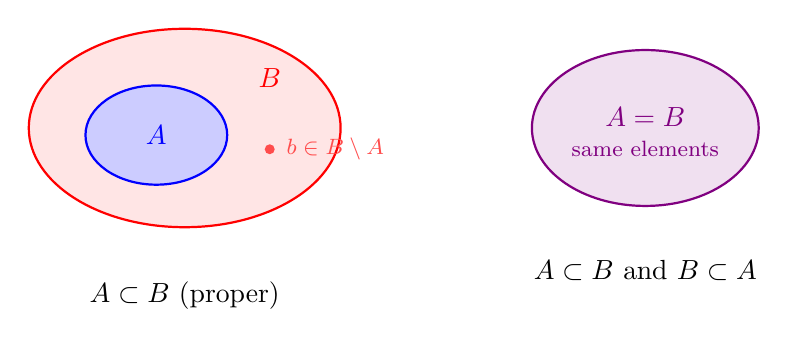
\begin{tikzpicture}[scale=0.9]
    % A proper subset of B
    \begin{scope}[xshift=0cm]
      \draw[thick, red, fill=red!10] (0,0) ellipse (2.2 and 1.4);
      \node[red] at (1.2,0.7) {$B$};
      \draw[thick, blue, fill=blue!20] (-0.4,-0.1) ellipse (1.0 and 0.7);
      \node[blue, font=\bfseries] at (-0.4,-0.1) {$A$};
      \fill[red!70] (1.2,-0.3) circle (2pt);
      \node[red!70, right, font=\footnotesize] at (1.3,-0.3) {$b \in B \setminus A$};
      \node[below=16pt] at (0,-1.4) {$A \subset B$ (proper)};
    \end{scope}
    % A = B
    \begin{scope}[xshift=6.5cm]
      \draw[thick, violet, fill=violet!12] (0,0) ellipse (1.6 and 1.1);
      \node[violet, font=\bfseries] at (0,0.15) {$A = B$};
      \node[violet, font=\footnotesize] at (0,-0.3) {same elements};
      \node[below=16pt] at (0,-1.1) {$A \subset B$ and $B \subset A$};
    \end{scope}
  \end{tikzpicture}
  \end{center}

  \note{
    Two sets "A" and "B" are defined to be equal if "A" is a subset of "B" and "B" is a subset of "A". In other words, they contain exactly the same elements. Otherwise, they are not equal. As you can see in the diagram on the left, when "A" is a proper subset of "B", "A" sits strictly inside "B", and there is at least one element in "B" that is not in "A". On the right, when "A" equals "B", the two sets coincide completely. This double-inclusion method of proving set equality, showing that each is a subset of the other, is one of the most common proof techniques in analysis.
  }
\end{frame}

% ============================================================
% DEFINITION 1.4 (progressive build)
% ============================================================

% --- Build 1/2: Definition ---
\begin{frame}{Definition 1.4: The Rationals $\mathbb{Q}$}
  \begin{defblock}{Definition 1.4}
    Throughout Chapter 1, the set of all rational numbers is denoted by $Q$.
  \end{defblock}

  \vspace{1em}
  \begin{hlbox}
    \[
      Q = \mathbb{Q} = \left\{ \frac{m}{n} : m, n \in \mathbb{Z},\; n \neq 0 \right\}
    \]
  \end{hlbox}

  \note{
    Definition 1.4 simply establishes notation: the letter "Q" will denote the set of all rational numbers throughout Chapter 1. These are all numbers of the form "m" over "n", where "m" and "n" are integers and "n" is not zero. Rudin uses a plain "Q" without the blackboard bold styling, but we will use the modern notation, blackboard bold "Q", interchangeably. This is our starting point, and the rest of the chapter builds from here.
  }
\end{frame}

% --- Build 2/2: What comes next ---
\begin{frame}{Definition 1.4: The Rationals $\mathbb{Q}$}
  \begin{defblock}{Definition 1.4}
    Throughout Chapter 1, the set of all rational numbers is denoted by $Q$.
  \end{defblock}

  \vspace{1em}
  \begin{hlbox}
    \[
      Q = \mathbb{Q} = \left\{ \frac{m}{n} : m, n \in \mathbb{Z},\; n \neq 0 \right\}
    \]
  \end{hlbox}

  \vspace{1em}
  \begin{hlbox}
    \textbf{What comes next:}
    \begin{itemize}
      \item \emph{Ordered sets} --- formalize the notion of ``$<$'' (Section 2)
      \item \emph{Fields} --- formalize arithmetic operations (Section 3)
      \item Build $\mathbb{R}$ from $\mathbb{Q}$ to fill the gaps (Section 4)
    \end{itemize}
  \end{hlbox}

  \note{
    This is the starting point for our construction. In the upcoming sections, we will define the general concepts of ordered set and field, which give us the language to describe the algebraic and order-theoretic structure of the rationals. Then, in Section 4, we will construct the real numbers by filling in the gaps that we discovered in Example 1.1.
  }
\end{frame}
}

{
\usebackgroundtemplate{%
  
\includegraphics[width=\paperwidth,height=\paperheight,keepaspectratio=false]{chapter_01_bg_05.png}%
}
% ============================================================
% SUMMARY (progressive build)
% ============================================================
\section{Summary}

% --- Build 1/5 ---
\begin{frame}{Summary}
  \begin{hlbox}
    \textbf{Key takeaways from this section:}
    \begin{itemize}
      \item Analysis needs a precise number system; $\mathbb{Q}$ is \emph{not} sufficient
    \end{itemize}
  \end{hlbox}

  \note{
    Let's review what we covered in this introduction. The main message is that the rational numbers are not sufficient for analysis. Despite seeming like a perfectly good number system, the rationals have fundamental gaps that prevent us from doing rigorous analysis. A proper treatment of convergence, continuity, and the other core concepts requires a number system that fills these gaps.
  }
\end{frame}

% --- Build 2/5 ---
\begin{frame}{Summary}
  \begin{hlbox}
    \textbf{Key takeaways from this section:}
    \begin{itemize}
      \item Analysis needs a precise number system; $\mathbb{Q}$ is \emph{not} sufficient
      \item \textbf{Example 1.1:} $\sqrt{2}$ is irrational (proof by contradiction)
    \end{itemize}
  \end{hlbox}

  \note{
    We proved in Example 1.1 that the square root of 2 is irrational, using a classic proof by contradiction. If "p" squared equals 2 and "p" equals "m" over "n", then both "m" and "n" must be even, contradicting our assumption.
  }
\end{frame}

% --- Build 3/5 ---
\begin{frame}{Summary}
  \begin{hlbox}
    \textbf{Key takeaways from this section:}
    \begin{itemize}
      \item Analysis needs a precise number system; $\mathbb{Q}$ is \emph{not} sufficient
      \item \textbf{Example 1.1:} $\sqrt{2}$ is irrational (proof by contradiction)
      \item The sets $A = \{p \in \mathbb{Q}^+ : p^2 < 2\}$ and $B = \{p \in \mathbb{Q}^+ : p^2 > 2\}$ have a \alert{gap} --- $A$ has no max, $B$ has no min
    \end{itemize}
  \end{hlbox}

  \note{
    We then saw that the sets "A" and "B" of positive rationals whose squares are less than or greater than 2 have a genuine gap between them, with no rational number sitting at the boundary. "A" has no maximum and "B" has no minimum.
  }
\end{frame}

% --- Build 4/5 ---
\begin{frame}{Summary}
  \begin{hlbox}
    \textbf{Key takeaways from this section:}
    \begin{itemize}
      \item Analysis needs a precise number system; $\mathbb{Q}$ is \emph{not} sufficient
      \item \textbf{Example 1.1:} $\sqrt{2}$ is irrational (proof by contradiction)
      \item The sets $A = \{p \in \mathbb{Q}^+ : p^2 < 2\}$ and $B = \{p \in \mathbb{Q}^+ : p^2 > 2\}$ have a \alert{gap} --- $A$ has no max, $B$ has no min
      \item \textbf{Remark 1.2:} Despite density, $\mathbb{Q}$ has gaps; $\mathbb{R}$ fills them
    \end{itemize}
  \end{hlbox}

  \note{
    Remark 1.2 emphasized that this gap exists despite the rationals being dense. The real number system is specifically constructed to fill these gaps, which is why it plays a fundamental role in analysis.
  }
\end{frame}

% --- Build 5/5 ---
\begin{frame}{Summary}
  \begin{hlbox}
    \textbf{Key takeaways from this section:}
    \begin{itemize}
      \item Analysis needs a precise number system; $\mathbb{Q}$ is \emph{not} sufficient
      \item \textbf{Example 1.1:} $\sqrt{2}$ is irrational (proof by contradiction)
      \item The sets $A = \{p \in \mathbb{Q}^+ : p^2 < 2\}$ and $B = \{p \in \mathbb{Q}^+ : p^2 > 2\}$ have a \alert{gap} --- $A$ has no max, $B$ has no min
      \item \textbf{Remark 1.2:} Despite density, $\mathbb{Q}$ has gaps; $\mathbb{R}$ fills them
      \item \textbf{Definitions 1.3--1.4:} Set membership ($\in$), subsets ($\subset$), equality, and the notation $Q$ for the rationals
    \end{itemize}
  \end{hlbox}

  \vspace{1em}
  \hl{\textbf{Coming up next:} Ordered Sets --- formalizing the relation ``$<$''}

  \note{
    Finally, we set up the basic set-theoretic language in Definitions 1.3 and 1.4 that will be used throughout the book: set membership, subsets, proper subsets, set equality, and the notation "Q" for the rationals. In the next section, we will formalize the notion of order, which is the first step toward understanding the structure of the real numbers.
  }
\end{frame}
}

\end{document}
